%!TEX root = 3-P_Masterdokument.tex
%!TEX encoding = UTF-8 Unicode
\chapter[Clause combining and complex clauses]{Clause combining and complex clauses}\label{sec:ComplexClauses}\is{complex sentence|(}

Complex sentences contain more than one predication. They typically consist of two (or more) clauses and are classically divided into two different main types: one type includes \isi{coordination} and the other one \isi{subordination}. Prototypically, coordinated clauses are semantically independent from each other, and this is reflected by the absence of \isi{dependency marking} of any sort. Subordinate clauses, on the other hand, are semantically dependent and marked for this dependency. Unfortunately, however, there is not always a clear correlation between semantic dependency and overt marking of this dependency. The boundaries between coordination and subordination are far from clear-cut, and there is rather a continuum which reaches from clauses that are semantically and syntactically independent on one end to semantically and syntactically dependent clauses on the other end and possibly a large number of clauses that fall inbetween these two poles  \citep[cf.][]{Lehmann1988}.\footnote{Actually the continuum goes even further in that semantically subordinate relations can also be expressed on the word-level thus reducing syntactic complexity again.} It is thus wise to think about semantic and syntactic dependency independently. 

In addition to complex sentences consisting of two (or more) clauses that may be semantically and syntactically more or less dependent on each other, there is another kind of complex clause formation in which one predication is neatly integrated into another one so that the result is a single clause with multiple verbs. An indication of this monoclausality is that only one possibility to negate\is{negation} the whole clause exists, with the negative particle having scope over both predicates (\citealp[cf.][299]{Haspelmath2016} in following \citealt[501]{Bohnemeyer2007}).

The case being complex like this, this chapter draws on the functional-semantic approach by \citet[]{Cristofaro2003} with regard to subordination.\is{subordination|(} According to this approach a subordinate clause lacks assertiveness and subordination is defined as “a situation of functional asymmetry whereby the profile of one of two linked SoAs [= state of affairs\footnote{In this work, I use the term “event” rather than “state of affair”. The latter term arose from a specific theoretical approach, i.e. Functional Grammar. The terminological distinction is not relevant here.}] is overriden by that of the other” \citep[39]{Cristofaro2003}. Clause combinations in which one clause lacks assertiveness are thus considered cases of subordination. Clause combinations in which both events are asserted are taken as cases of \isi{coordination}. This is illustrated by (\ref{ex:new23-subord}) and (\ref{ex:new23-coord}). The first one is a conditional clause, thus the realisation of the consequence clause is marked as dependent on the realisation of the antecedent – or rather non-realisation in this case because the predicate is negated. In any case, the consequent clause is non-asserted due to its dependence on the antecedent.

The example comes from Juan Ch. speaking about the \textit{patrón}, who was expected to arrive the next day in order to distribute some goods.

\ea\label{ex:new23-subord}
\begingl
\glpreamble kue kuina kapunuina repente sabado kapunuinakena\\
\gla kue kuina kapunu-ina repente sabado kapunu-ina-kena\\
\glb if \textsc{neg} come-\textsc{irr.nv} maybe Saturday come-\textsc{irr.nv}-\textsc{uncert} \\
\glft ‘if he doesn’t come (tomorrow), maybe he comes on Saturday’
\endgl
\trailingcitation{[nxx-p630101g-1.066]}
\xe

\is{subordination|)} 

In (\ref{ex:new23-coord}), however, Juana presents both propositions as asserted as indicated by the use of the connective \textit{i} ‘and’. This is also verified by how she presents the issue in Spanish (switching back and forth between Paunaka and Spanish while talking with me). She speaks about her daughter here who had promised to visit her in Bolivia and then take her to Spain for a visit.

\ea\label{ex:new23-coord}
\begingl
\glpreamble kapupunuina i tumanÿ\\
\gla kapupunu-ina i ti-uma-nÿ\\
\glb come.back-\textsc{irr.nv} and 3i-take.\textsc{irr}-1\textsc{sg}\\
\glft ‘she will come back and take me (to Spain)’
\endgl
\trailingcitation{[jxx-p110923l-1.258]}
\xe

It is further possible to distinguish between different types of subordinate\is{subordination} relations in Paunaka: adverbial relations\is{adverbial relation|(} (as in (\ref{ex:new23-subord})), complement relations,\is{complement relation} and relative relations.\is{relative relation} The clauses expressing an adverbial relation are consequently called adverbial claus\-es, complement relations are expressed by complement clauses and relative relations by relative clauses. Adverbial clauses modify a verb or clause, complement clauses are required as arguments\is{argument} by some verbs, relative clauses modify an argument or, in the case of headless relative clauses, become an argument themselves. This does not imply that there is a 1:1 correspondence between function and form, at least not in Paunaka, and differently formed clauses may fulfil one and the same function.\is{adverbial relation|)}

The morphosyntactic repertoire to combine clauses and to form complex single clauses includes asyndetic juxtaposition, syndetic juxtaposition (with independent words functioning as linkers as in (\ref{ex:new23-subord}) and (\ref{ex:new23-coord})), dependency marking on the verb and deranking. All of them will be explained in more detail below (see \sectref{sec:TypesClauseCombining}).

Predicates in coordinate\is{coordination} clauses are never marked for dependency in any way, but there may be a \isi{connective} word that specifies the kind of relation between the clauses, in (\ref{ex:new23-coord}) this is \textit{i} ‘and’. Among coordinate relations are temporal sequence, conjunction,\is{conjunctive} disjunction,\is{disjunctive} \isi{adversative} and onsequence.\is{consecutive} Alternatively, the clauses can be juxtaposed asyndetically,\is{juxtaposition} i.e. without any morphosyntactic linking device.\is{syndesis/asyndesis}

As regards coding of \isi{subordination},\is{verb|(} three strategies prevalent in Amazonian languages\is{Amazonian language} have been identified by \citet[10]{Gijnetal2011}. They build on nominalisation,\is{grammatical nominalisation} combination of verbs or close integration of different verbs into one clause or even into one verb as given in \figref{fig:SubordinationSouthAmerica}.


\begin{figure}[!ht]

\begin{enumerate}
\item Nominal strategies: the subordinate verb is nominalized, possibly with the retention of (some) verbal categories.
\item Verbal strategies: clause combination of two more or less finite structures, often with a (bound) dependency marker
\item Integrating strategies: the two predicative elements are grammatically integrated, resulting in multi-verb constructions, verb compounds, and affixing.
\end{enumerate}
\caption{Subordination strategies in South America \citep[10]{Gijnetal2011}}
\label{fig:SubordinationSouthAmerica}

\end{figure}


In Paunaka’s subordinate clause formation, we can observe all of these strategies to a certain degree.\is{subordination|(}  

As for verbal strategies, the verb in the subordinate clause is totally finite,\is{finite verb|(} in the sense that all categories obligatorily expressed on a main clause predicate, i.e. person\is{person marking} and RS,\is{reality status|(} are expressed in the same way on the subordinate predicate and there is no dependency marker. This does not preclude that the RS of the subordinate predicate is in some cases determined by the main clause predicate\is{reality status|)} or that certain TAME markers on the subordinate predicate provide clues for the interpretation about the specific semantic connection to the main clause. A subordinate clause with a finite verb not marked for dependency, i.e. a verb that is “balanced” to use the terminology of \citet[]{Cristofaro2003}, can be juxtaposed to a main clause without any specific linking device. This is regarded as asyndetic \isi{juxtaposition}.\is{syndesis/asyndesis} (\ref{ex:new23-rel24}) provides an example of an asyndetically juxtaposed relative clause. The verb of the main clause is \textit{tikijaneyu} ‘they are many’ and its subject is \textit{chipeunube baka} ‘their cows’. This subject is modified by \textit{tipabenteikunube} ‘they sell (them)’. That the second verb is connected to the preceding clause is signalled by the intonation, but the exact relationship to it has to be deduced from the context. It is not shown on the verb nor anywhere else in the clause, i.e. an independent clause with the meaning ‘they sell (them)’ would have exactly the same structure. The sentence comes from Juana speaking about her grandparent’s journey to Moxos to buy cows.

\ea\label{ex:new23-rel24}
\begingl
\glpreamble tikijaneyu chipeunube baka tipabenteikunube\\
\gla ti-kijane-yu chi-peu-nube baka ti-pabenteiku-nube\\
\glb 3i-be.many-\textsc{ints} 3-animal-\textsc{pl} cow 3i-sell-\textsc{pl}\\
\glft ‘there are a whole lot of cows that they sell’
\endgl
\trailingcitation{[jxx-e150925l-1.211]}
\xe


If there is a linker but no sign of dependency on the subordinate verb itself, I take it as a case of syndetic \isi{juxtaposition}, as in (\ref{ex:new23-subord}) above, where \textit{kue} ‘if, when’ signals that we are dealing with a conditional sentence or one including temporal overlap. Linkers are usually independent words that introduce the subordinate clause. In adverbial clauses,\is{adverbial relation} we find connectives,\is{connective} in relative clauses,\is{relative relation} there are nominal demonstratives,\is{nominal demonstrative} and in complement clauses\is{complement relation} we marginally find demonstratives,\is{nominal demonstrative}\is{complementiser} too. 

Regarding integrating strategies, these are found in complementation,\is{complement relation} such as in (\ref{ex:new23-compl}), and also for verbal expressions of goals of motion predicates,\is{motion predicate} i.e. constructions expressing \isi{purpose} of motion. The subordinate verbs in complementation are usually completely unmarked for dependency, in the expression of purpose of motion, we find two different construction types, one in which there is no sign of dependency either (\isi{serial verb construction}) and one in which dependency is marked\is{dependency marking} on the purpose verb (\isi{motion-cum-purpose construction}). 

(\ref{ex:new23-compl}) comes from Clara asking María C. about her knowledge in Napeka.\footnote{María C.’s father was a speaker of Napeka, but he died when she was still very young.}

\ea\label{ex:new23-compl}
\begingl
\glpreamble ¿pichuna pichujiku napeka?\\
\gla pi-chuna pi-chujiku napeka\\
\glb 2\textsc{sg}-be.capable 2\textsc{sg}-speak Napeka\\
\glft ‘do you speak Napeka?’ (lit.: ‘are you capable to speak Napeka?’)
\endgl
\trailingcitation{[cux-c120414ls-2.272]}
\xe
\is{finite verb|)}

%kuina naichuna nisuika, jxx-e110923l-2.149
%pichuna pichujiku eka paunaka, jxx-p120515l-1.160

Distinctly nominal strategies are rare in Paunaka, but see \sectref{sec:SyntaxNominalisation} for some examples including nominalised verbs that have shown up in the corpus. More importantly, there is one form of the verb that I call “deranked”\is{deranked verb|(} throughout this grammar, using the terminology by \citet[]{Cristofaro2003}, which has partly verbal and partly nominal characteristics. It seems that at least in some constructions such a deranked verb is chosen because a (more) nominal word is demanded. Regarding the partly nominal behaviour of deranked verbs, this is bound to these verbs not expressing the category of person in exactly the same way as main clause predicates do, but rather like (internal) possessors\is{possessor} of inalienable nouns. This fact should not be overemphasised, though, because subject markers on verbs and possessor markers on nouns are identical except for one third person marker that is only found with verbs.\is{person marking} The use of such a deranked verb is the strongest sign for \isi{embedding} in Paunaka, i.e. the clause containing the deranked verb is dependent, it cannot usually occur on its own \citep[cf.][]{Lehmann1988}.\footnote{See, however, \sectref{sec:AdverbialModification} for clauses in which the deranked verb is the only verb.}\is{deranked verb|)}\is{subordination|)}

The remainder of this chapter is organised around the functional-semantic subclasses of complex sentences and clauses that are traditionally distinguished, coordination (\sectref{sec:Coordination}), adverbial relations (\sectref{sec:AdverbialClauses}), complement relations (\sectref{sec:ComplementClauses}) and relative relations (\sectref{sec:RelativeClauses}). In addition, a focus construction containing a deranked verb is discussed in \sectref{sec:AdverbialModification}. Before giving details about these different sub-classes of clause combinations and complex clauses, the different construction types found throughout this chapter are presented in greater detail in \sectref{sec:TypesClauseCombining}. This has the advantage that the same construction types do not have to be explained over and over again, when occurring in different contexts.

\section[Construction types in clause combining and complex clause formation]{Construction types in clause combining and\newline complex clause formation}\label{sec:TypesClauseCombining}

When considering the combination of clauses and predicates, five general features turn out to be important in Paunaka: integration, syndesis,\is{syndesis/asyndesis} \isi{dependency marking}, deranking,\is{deranked verb} and predetermination of the RS.\is{reality status} These features correspond to five general questions given in \figref{fig:SubordinationQuestions}.

\begin{figure}[!ht]
\centering
\begin{center}
\begin{itemize}
\item Integration: Are both predicates individually negatable?
\item Syndesis: Is the kind of relation marked on one of the clauses?
\item Dependency marking: Is one of the verbs marked for dependency?
\item Deranking: Has one of the verbs acquired some nominal properties?
\item Reality status: Is the RS of one of the verbs predetermined by its relation to the other verb?
\end{itemize}
\caption{Questions to determine the relation between two clauses or predicates}
\label{fig:SubordinationQuestions}
\end{center}
\end{figure}


Considering the overt encoding of relations only, i.e. the features syndesis, dependency marking and deranking, it turns out that there are three different general construction types and one minor one in clause combining and complex clause formation. I call them asyndetic \isi{juxtaposition}, syndetic \isi{juxtaposition}, \isi{dependency marking} and deranking.\is{deranked verb}\is{syndesis/asyndesis} These four types cross-cut the different functional categories of complex sentences in Paunaka, which are \isi{coordination}, adverbial relations,\is{adverbial relation} complement relations,\is{complement relation} and relative relations.\is{relative relation} This means that there is usually no one-to-one correspondence between construction type and functional type of the complex sentence, but it also not the case that that each of the functional types is found with all construction types. In \tabref{table:ClauseCombiningConstructions}, the construction types are ordered from least overt marking of dependency to most overt marking of dependency (first column). Thus the construction type that includes no overt morphosyntactic marking of \isi{coordination} or \isi{subordination}, i.e. asyndetic juxtaposition, is positioned on top of the table. Syndetic juxtaposition occupies a middle position. In this construction type, a \isi{connective} specifies the kind of relation between the two clauses.\is{syndesis/asyndesis} This is followed by \isi{dependency marking}, which applies to only one specific construction. The dependent verb is non-controversially verbal. This is different in deranking. The \isi{deranked verb} is partly verbal and partly nominal, which eases its \isi{embedding} into the clause. Since deranking predominantly occurs in \isi{subordination} contexts, we can consider it a sign of dependency marking. It is thus found at the bottom of the table. 

All three main construction types are found in clause combining as well as in complex monoclausal constructions, and the fourth one (\isi{dependency marking}) is only found in one complex monoclausal construction. I provide more detailed descriptions for each construction type below. Having identified the different construction types, it is still necessary to check for degree of integration and predetermination of RS of each construction. This will be done in the individual sections on coordinate and subordinate relations, whenever possible. 


\begin{sidewaystable}
\caption{Construction types in clause combining}

\begin{tabularx}{\textwidth}{QlQQl}
\lsptoprule
Construction type & Independent negation & Type of relation & Comment & Sections\cr
\midrule
asyndetic juxtaposition & yes & coordination & & \sectref{sec:AsyndeticCoordination}  \cr
& & adverbial relations\is{adverbial relation} & & \sectref{sec:AsyndeticSubordination}\cr
& & relativisation & typically headed & \sectref{sec:UnmarkedRC}\cr
& no & complementation & & \sectref{sec:Unmarked_CCs} \cr
& & adverbial relations\is{adverbial relation} & only purpose of motion & \sectref{sec:SerialVerbs}\cr
syndetic juxtaposition & yes & coordination & & \sectref{sec:SequentialCoordination}--\ref{sec:ConsecutiveCoordination}\cr
 & & adverbial relations\is{adverbial relation} & & \sectref{sec:AC-kue}--\ref{sec:AprenhensionalClauses}\cr
 & & complementation & marginal type & \sectref{sec:CC_CMPL} \cr
 & & relativisation & typically headless & \sectref{sec:HeadlessRC}\cr
 dependency marking & no & adverbial relations\is{adverbial relation} & only purpose of motion & \sectref{sec:MotionCumPurpose} \cr
 deranking & yes & adverbial relations\is{adverbial relation} & & \sectref{sec:SubordinateACs} \cr
& & relativisation & mainly of obliques & \sectref{sec:RC-Subord} \cr
& no & complementation & atypical relations & \sectref{sec:CCs_deranked}\cr
& & focus construction  &  subtype of equative clause & \sectref{sec:AdverbialModification} \cr
\lspbottomrule
\end{tabularx}
\label{table:ClauseCombiningConstructions}
\end{sidewaystable}


\subsection{Asyndetic juxtaposition}\label{sec:AsyndeticJuxtaposition}
\is{syndesis/asyndesis|(}
\is{juxtaposition|(}

The linking of two clauses can be totally unmarked, i.e. there is neither a connective word of any kind nor does one of the predicates have a special form or carry a marker with a peculiar linking function. This is not to say that there is absolutely no means to express the relation between the clauses, on the contrary, TAME markers\is{tense}\is{aspect}\is{modality}\is{evidentiality} on the predicates often provide the clue as to how to analyse the relation between the clauses. It is just that these markers are not specified for clause linking, they can also occur when no linking is involved.

Asyndetic juxtaposition is frequently found in \isi{coordination} of semantically independent clauses, called “parataxis” by \citet[]{Lehmann1988}, but also in \isi{subordination}, where we recognise that one clause is pragmatically subordinate to the other one without this being marked overtly \citep[cf.][355]{Mithun1988}. This is the case with most complement\is{complement relation} and headed\is{head} relative clauses\is{relative relation} as well as some adverbial clauses.\is{adverbial relation}

As for integration of the two predications into a single clause, this is different for each relation and construction as shown by \figref{fig:IntegrationScaleAsyndeticJuxtaposition} inspired from the diagram given by \citet[307]{Payne1997}. 

\begin{figure}
\centering
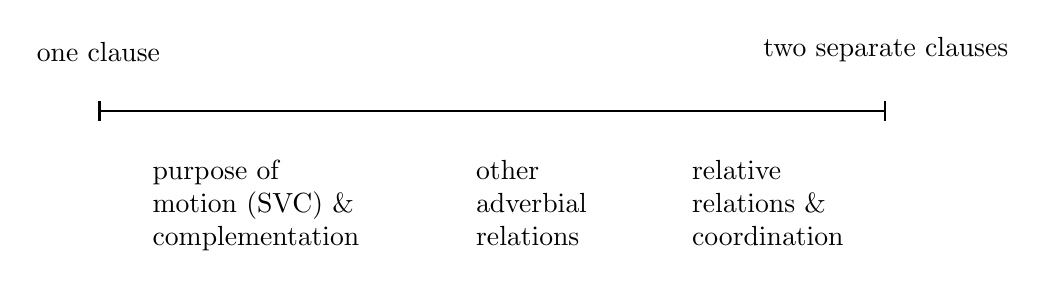
\begin{tikzpicture}
\draw [thick] [|-|]  (0,0) -- (10,0);
\node[align=left, above] at (0.0, .5){one clause};%
\node[align=right, above] at (10.0, .5){two separate clauses};%

\node[align=left, below] at (2.0,-.5)%
    {purpose of\\motion (SVC) \&\\complementation};
\node[align=left, below] at (5.5,-.5)%
    {other\\adverbial\\relations};
\node[align=left, below] at (8.5,-.5)%
    {relative\\relations \&\\coordination};
\end{tikzpicture}
\caption{Integration of asyndetically juxtaposed clauses}
\label{fig:IntegrationScaleAsyndeticJuxtaposition}
\end{figure}

It can be claimed that all coordinated\is{coordination} clauses and all headed\is{head} relative clauses\is{relative relation} that are asyndetically juxtaposed to another clause have a relatively high degree of independence. Nonetheless, these clauses are not totally independent or separate, because they occur in a single \isi{intonation} unit together with the clause they are combined with. On the other hand, in complementation\is{complement relation} as well as in expressions of \isi{purpose} of motion the subordinate clause lacks independent negatability,\is{negation} a sign that it is neatly integrated into the main clause (and thus perhaps not a “clause” at all). Other types of asyndetically juxtaposed adverbial clauses\is{adverbial relation} are closer to the biclausal end of the continuum than to the monoclausal one, but they are not as independent as coordinated\is{coordination} and headed relative clauses.\is{relative relation} This is bound to the fact that the RS\is{reality status} of the subordinate predicate\is{subordination} is sometimes determined in some way by the main clause predicate. Irrealis RS\is{irrealis} is necessarily found in adverbial clauses\is{adverbial relation} of the \isi{purpose} (except for purpose of motion), \isi{apprehensional} and counterfactual\is{counterfactuality} conditional types. Irrealis RS is also found in complement clauses\is{complement relation} of desiderative and manipulative predicates.\is{manipulative verb}\is{desiderative verb} The RS\is{reality status|(} of the subordinate predicate must match the one of the matrix predicate in complement clauses of knowledge and perception predicates. In purpose-of-motion expressions, RS of the \isi{purpose} predicate has to be either irrealis or identical to the motion verb.\is{reality status|)}\is{motion predicate}

(\ref{ex:Asycoor-2}) provides an example of two clauses that are coordinated by asyndetic juxtaposition. There is no sign of connection between the clauses, but the reportive marker\is{evidentiality} \textit{-ji} that occurs twice gives a hint in this case that we are probably dealing with two clauses, since it usually occurs only once per clause (but may also occur twice in one clause, so that this is indeed only a hint and no reliable evidence). 

The example comes from Juana’s account about her criminal in-law. He hid away in the forest, but came home at night to eat and sleep until he was arrested one night.

\ea\label{ex:Asycoor-2}
\begingl
\glpreamble bueno, tibÿkuputuji tinikuji\\
\gla bueno ti-bÿkupu-tu-ji ti-niku-ji\\
\glb well 3i-enter-\textsc{iam}-\textsc{rprt} 3i-eat-\textsc{rprt}\\
\glft ‘well, he came in and ate, it is said’
\endgl
\trailingcitation{[jxx-p120430l-2.147-148]}
\xe

%\ea\label{ex:Asycoor-222}
%\begingl
%\glpreamble upujaine echÿu kupeitu tiyunuji tiniku mantarina naukuji\\
%\gla upu-jai-ne echÿu kupei-tu ti-yunu-ji ti-niku mantarina nauku-ji\\
%\glb other-day-\textsc{possd} \textsc{dem}b afternoon-\textsc{iam} 3i-go-\textsc{rprt} 3i-eat tangerine there-\textsc{rprt}\\
%\glft ‘the other day in the afternoon he went, it is said, and ate a tangerine there, it is said’\\
%\endgl
%\trailingcitation{[jxx-p120430l-2.420-421]}
%\xe
%not so sure whether this is not a SVC in the end... 


For contrast with the coordinated clauses in (\ref{ex:Asycoor-2}) above, consider (\ref{ex:Asysub-1}) below, which encodes a subordinate relation, a complement clause whose predicate \textit{tinika} is also completely unmarked for linkage to the matrix predicate, but has to occur with \isi{irrealis} RS. The example was elicited from María S. and refers to her coati, which was chasing a butterfly.

 \ea\label{ex:Asysub-1}
\begingl
\glpreamble tisachu tinika churupepe\\
\gla ti-sachu ti-nika churupepe\\
\glb 3i-want 3i-eat.\textsc{irr} butterfly\\
\glft ‘it wants to eat the butterfly’
\endgl
\trailingcitation{[rxx-e150220s-1.20]}
\xe

There is little ambiguity about how to analyse the relations in the constructions that show a high degree of integration like complement clauses\is{complement relation} and serial verb constructions.\is{serial verb construction} In \isi{coordination} and in most expressions of adverbial relations,\is{adverbial relation} however, one clause is attached to another one at a higher level, the sentence. If the kind of relation between both clauses is not overtly marked by a connective, it is sometimes hard to determine whether a speaker wants to present both events as being asserted, i.e. coordinated, or one of the events as non-asserted and pre-supposed, i.e. in an \isi{adverbial relation} to the other one. It may sometimes even be the case that a clause could alternatively be analysed as a coordinated, adverbial or relative clause.

This is the case in (\ref{ex:CoC-AC-RC}). Both clauses can either be understood to represent two equally asserted facts that contribute to the realisation of the two old ladies that Juana is a speaker of Paunaka or alternatively the second clause (about understanding Paunaka) may offer the basis for the deduction expressed in the first clause or it can be analysed as a relative clause to modify a participant of the main clause. If we favour the first analysis, this is an example of \isi{coordination}, the second analysis yields an adverbial clause\is{adverbial relation} and according to the third one, we deal with relativisation here.

The sentence was produced by Juana, when she told me of an encounter with two old ladies in Candelaria who first did not recognise that she was a speaker of Paunaka.


\ea\label{ex:CoC-AC-RC}
\begingl
\glpreamble “kumade, biparienteneyenu eka pimiya chisamuyenu paunaka”\\
\gla kumade bi-pariente-ne-yenu eka apimiya chi-samu-yenu paunaka\\ 
\glb fellow 1\textsc{pl}-relative-\textsc{possd}-\textsc{ded} \textsc{dem}a girl 3-hear-\textsc{ded} Paunaka\\ 
\glft ‘“fellow, this girl must be our relative (and) she must understand Paunaka!”’ \\ or: ‘“fellow, this girl must be our relative, since apparently she understands Paunaka”’ \\or: ‘“fellow, this girl who apparently understands Paunaka must be our relative”’
\endgl
\trailingcitation{[jxx-p120515l-1.108]}
\xe

Even if we decide to analyse a clause as encoding an \isi{adverbial relation}, it is still not always clear which kind of adverbial relation is encoded as in (\ref{ex:temp-cause}), which may express a temporal (“when”) or a causal (“because”) relation. This ambiguity is also reflected in the English translation with a gerund, which leaves the specific kind of semantic connection unexpressed, just like the Paunaka predicate does. However, while the predicate in the English translation is deranked, there is no sign of dependency in the original Paunaka clause.\footnote{The translation fails to capture another peculiarity: the verb in the adverbial clause of the Paunaka example, besides not involving passivisation like the English translation, has no object marker and is thus best analysed as encoding the event in such a way that children went around and invited other children to come to school, i.e. it was not only Miguel who was invited.} The sentence stems from Miguel’s account about how he learned to read, write and calculate.

\ea\label{ex:temp-cause}
\begingl
\glpreamble komensau niyunu xhikuerayae tikupirauchunube eka punachÿ sesejinube\\
\gla komensau ni-yunu xhikuera-yae ti-kupirauchu-nube eka punachÿ sesejinube\\
\glb begin 1\textsc{sg}-go school-\textsc{loc} 3i-invite-\textsc{pl} \textsc{dem}a other children\\
\glft ‘I started to go to school being invited by other children’
\endgl
\trailingcitation{[mxx-p181027l-1.003]}
\xe

%- not clear whether coordinate or adverbial clause: jxx-p120430l-2.236, 

The question of which type of clause connection we are dealing with is of concern for translation into English, where the kind of relation between the events often needs to be expressed overtly, and it is of concern when trying to attach some labels to the examples in this grammar and sort them into different categories. It is, of course, not of concern for the speakers of Paunaka, who do not demand this kind of analysis, when speaking their language. They simply link by \isi{intonation} what belongs together.

\subsection{Syndetic juxtaposition}\label{sec:SyndeticJuxtaposition}\is{connective|(}

In syndetic juxtaposition, the predicates of both clauses are balanced,\is{finite verb} just like in asyndetic juxtaposition, but there is a linking element that specifies the kind of relation between the clauses. %These clauses have also been called adjoined clause \citep[185]{Lehmann1988}.
In Paunaka, we find syndetic juxtaposition in \isi{coordination} and in adverbial linking.\is{adverbial relation} A connective is placed between the two clauses in these cases. There is always only one connective word per connection, so we can speak of a monosyndetic pattern \citep[cf.][4]{Haspelmath2004}. We can also speak of syndetic juxtaposition in defining the construction type of most headless and a few headed\is{head} relative clauses\is{relative relation} and of a marginal type of complement clauses.\is{complement relation}\is{complementiser} However, in these cases, it is not a connective but a nominal demonstrative that serves as linker.

On the integration scale given in \figref{fig:IntegrationScaleSyndeticJuxtaposition}, syndetic complementation is possibly found far on the left-hand side, and I use the word “possibly” here, because this is really a marginal type of complementation, so that I cannot provide much information about it. Headless relative clauses share with complement clauses that they are integrated into the main clause as an argument.\is{argument} However, in contrast to complement clauses, headless relative clauses can be negated separately.\is{negation} Relative relations\is{relative relation} are thus placed right of complementation. Adverbial relations\is{adverbial relation} and \isi{coordination} are found at the right side of the scale. However, since adverbial clauses lack assertiveness, they are less independent than coordinated clauses. Since in syndetic juxtaposition both of them are overtly linked to another piece of discourse, they are both less independent than the asyndetically juxtaposed ones.

\begin{figure}
\centering
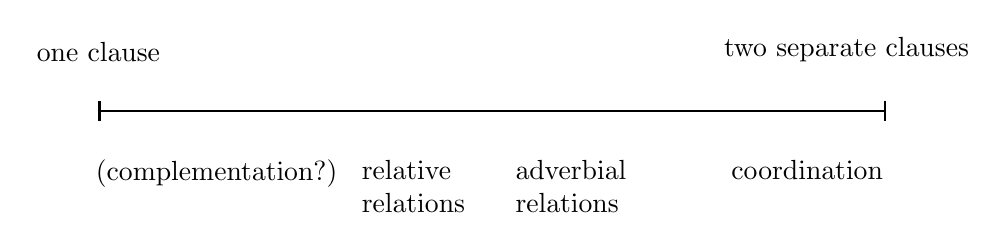
\begin{tikzpicture}
\draw [thick] [|-|]  (0,0) -- (10,0);
\node[align=left, above] at (0.0, .5){one clause};%
\node[align=right, above] at (9.5, .5){two separate clauses};%

\node[align=left, below] at (1.5,-.5)%
    {(complementation?)};
\node[align=left, below] at (4,-.5)%
    {relative\\relations};
\node[align=left, below] at (6,-.5)%
    {adverbial\\relations};
\node[align=left, below] at (9,-.5)%
    {coordination};
\end{tikzpicture}
\caption{Integration of syndetically juxtaposed clauses}
\label{fig:IntegrationScaleSyndeticJuxtaposition}
\end{figure}


As for \isi{coordination} and adverbial relations,\is{adverbial relation} there is no ambiguity as to which kind of semantic relation between the clauses is expressed, since there are several different connectives (see \sectref{sec:Conjunctions} for an overview of connective words). (\ref{ex:Syn-te-1}) involves coordination with the sequential connective \textit{te}. Like (\ref{ex:Asycoor-2}) above, it is about the last things Juana’s brother did before he suddenly died. 

\ea\label{ex:Syn-te-1}
\begingl
\glpreamble titupunubu terminalyae te tiyunu mikroyae\\
\gla ti-tupunubu terminal-yae te ti-yunu mikro-yae\\
\glb 3i-arrive bus.station-\textsc{loc} \textsc{seq} 3i-go microbus-\textsc{loc}\\
\glft ‘he arrived at the bus station and then went by microbus’
\endgl
\trailingcitation{[jxx-p120430l-2.402]}
\xe

In (\ref{ex:Syn-kue-2}) on the other hand, we have a subordinate clause, which is introduced by the connective \textit{kue} ‘if, when’. This connective marks the clause as an antecedent in a conditional sentence. The verb in the antecedent clause is not marked for subordination, but it necessarily takes \isi{irrealis} RS, since it refers to a non-factual event. The sentence was produced by Miguel, when inviting María C. to come to the workshop on Paunaka we had organised in 2011. Her husband was very ill, so she doubted that she would be able to come. Miguel was also sure that María C.’s husband could not stay at home alone.

\ea\label{ex:Syn-kue-2}
\begingl
\glpreamble kue piyuna tiyunauku echÿu\\
\gla kue pi-yuna ti-yuna-uku echÿu\\
\glb if 2\textsc{sg}-go.\textsc{irr} 3i-go.\textsc{irr}-\textsc{add} \textsc{dem}b\\
\glft ‘if you go, he has to go, too’
\endgl
\trailingcitation{[mux-c110810l.042]}
\xe

In some relative clauses,\is{relative relation} typically the headless ones, the linking element is a \isi{nominal demonstrative}, thus it is not specialised as a connective per se. The demonstrative precedes the otherwise completely unmarked clause just like it would precede a noun. This can be considered as a sign of the verb having gained some nominal characteristics. (\ref{ex:Syn-REL}) offers one example.

María C. asks Miguel here about a sheet of paper with some information about our project that Federico had given her a few days earlier.

\ea\label{ex:Syn-REL}
\begingl
\glpreamble ¿i kena echÿu chinejiku ukuinebu?\\
\gla i kena echÿu chi-nejiku ukuinebu\\
\glb and \textsc{uncert} \textsc{dem}b 3-leave some.time.ago\\
\glft ‘and what about the one he left some days ago?’
\endgl
\trailingcitation{[mux-c110810l.131]}
\xe
\is{connective|)}
\is{juxtaposition|)}
\is{syndesis/asyndesis|)}

\subsection{Dependency marking}\label{sec:ConstructionTypePA}

\is{subordination|(}
\is{dependency marking|(}
There is only one specific construction in which a \isi{finite verb} carries a dependency marker: the motion-cum-purpose construction,\is{motion-cum-purpose construction|(} in which the purpose verb is marked by the dislocative marker\is{dislocative|(} (see \sectref{sec:PA}). Although it mostly occurs within this construction, the marker is also found in other contexts that have nothing to do with dependency. It may have had primarily functions not related to subordination in older times, but this is relatively restricted today. In the motion-cum-purpose construction, the verb expressing purpose is dependent on the one expressing motion by having the same subject and the same RS. Thus, the dislocative marker can be considered a marker of this dependency. The dislocative marker occurs directly after the verb stem, but does not cause deletion of the thematic suffixes. It inflects for RS.\is{dislocative|)} 

Since the purpose verb in a motion-cum-purpose construction cannot be negated individually,\is{negation} the construction belongs to the integrating monoclausal type, see \figref{fig:IntegrationScaleMCPC}.

\begin{figure}
\centering
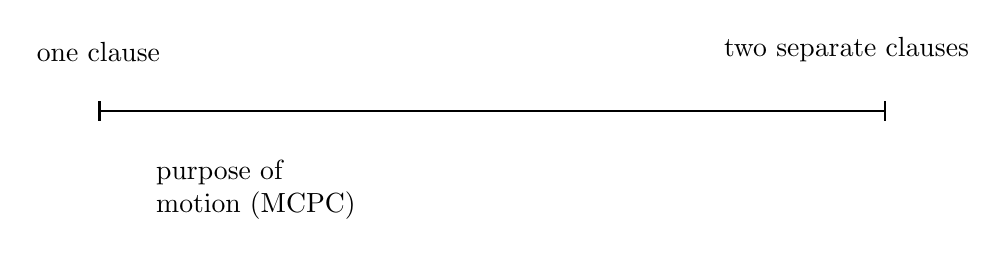
\begin{tikzpicture}
\draw [thick] [|-|]  (0,0) -- (10,0);
\node[align=left, above] at (0.0, .5){one clause};%
\node[align=right, above] at (9.5, .5){two separate clauses};%
\node[align=left, below] at (2.0,-.5)%
    {purpose of\\motion (MCPC)};
\end{tikzpicture}
\caption{Integration of verbs marked for dependency}
\label{fig:IntegrationScaleMCPC}
\end{figure}

A motion predicate,\is{motion predicate} most typically the verb \textit{-yunu} ‘go’, is combined with another verb that encodes the purpose of the motion. The purpose verb carries the \isi{dislocative} marker and is thus marked as dependent, but does not have any nominal properties in contrast to the deranked subordinate verb (see \sectref{sec:Subordination-i} below). One example of a motion-cum-purpose construction is (\ref{ex:MOC-1}). It was elicited from Miguel.

\ea\label{ex:MOC-1}
\begingl
\glpreamble niyuna ninikupa\\
\gla ni-yuna ni-niku-pa\\
\glb 1\textsc{sg}-go.\textsc{irr} 1\textsc{sg}-eat-\textsc{dloc.irr}\\
\glft ‘I will go to eat’
\endgl
\trailingcitation{[mxx-e160811sd.174]}
\xe
\is{motion-cum-purpose construction|)}

If we exchange the verb containing the dislocative marker by one with the subordinate suffix \textit{-i}, the meaning of the sentence changes. Compare to (\ref{ex:noMOC}), which was also elicited from Miguel.

\ea\label{ex:noMOC}
\begingl
\glpreamble niyuna ninikia\\
\gla ni-yuna ni-nik-i-a\\
\glb 1\textsc{sg}-go.\textsc{irr} 1\textsc{sg}-eat-\textsc{subord}-\textsc{irr}\\
\glft ‘I will go in order to eat’
\endgl
\trailingcitation{[mxx-e160811sd.176-177]}
\xe

In (\ref{ex:MOC-1}) motion is directed towards the place where the food is, and this is not necessarily the case in (\ref{ex:noMOC}), which only specifies that the speaker moves from or to a place and that the purpose for this motion is eating, but the exact relation between going and eating is not specified. Actually, though grammatically correct, speakers would normally not use a sentence like (\ref{ex:noMOC}), exactly because the relation between both predicates is too vague. The use of deranked verbs with the subordinate suffix \textit{-i} is the topic of the next section.
\is{dependency marking|)}

\subsection{Deranking}\label{sec:Subordination-i}
\is{deranked verb|(}

Active verbs can be marked as subordinate by a suffix \textit{-i}.\is{active verb}\footnote{Stative verbs do usually not take this suffix, but there are a few exceptions in the corpus, as well as a few cases in which a non-verbal predicate\is{non-verbal predication} takes the subordinate marker, e.g. the non-verbal predicate\is{motion predicate} \textit{kapunu} ‘come’ sometimes has a subordinate form \textit{kapuniu}. This shows shows how pervasive the pattern has become.} Verbs that take \textit{-i} partly lose their verbal properties. They are deranked. Deranked verbs occur in different kinds of adverbial clauses,\is{adverbial relation} in a few atypical complement clauses,\is{complement relation} in the relativisation of obliques\is{oblique} and in a specific focusing construction\is{focus} (including some questions).\is{interrogative clause} They sometimes also simply pop up for no apparent reason -- or at least no reason obvious to me. The suffix \textit{-i} can thus be considered a multi-purpose subordinator. The different constructions with a deranked verb occupy different positions on the integration scale as is illustrated in \figref{fig:IntegrationScaleDeranking}. In \isi{focus} constructions and complementation,\is{complement relation} the deranked verb constitutes an \isi{argument} and is thus completely integrated. In relative\is{relative relation} and adverbial clauses\is{adverbial relation} it acts as a modifier and as such it is also individually negatable.\is{negation} Since the clause with the deranked verb could not occur independently in this way, they occupy a middle position on the scale.

A clause with a deranked verb usually contains no other means to establish the link to another clause. Occasionally, however, we find it being combined with a \isi{preposition} in adverbial clauses\is{adverbial relation} or with a demonstrative\is{nominal demonstrative} in relative clauses.\is{relative relation} 

\begin{figure}
\centering
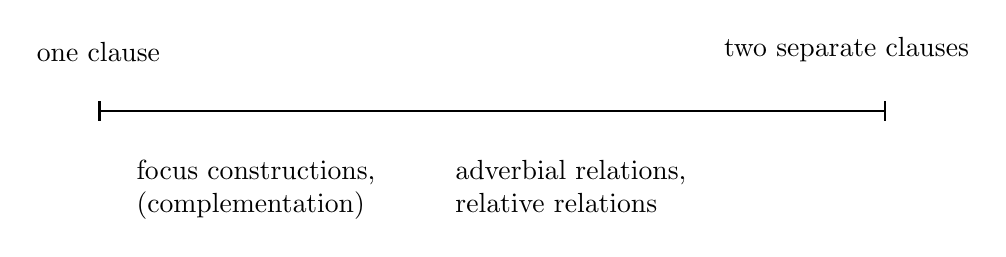
\begin{tikzpicture}
\draw [thick] [|-|]  (0,0) -- (10,0);
\node[align=left, above] at (0.0, .5){one clause};%
\node[align=right, above] at (9.5, .5){two separate clauses};%
\node[align=left, below] at (2.0,-.5)%
    {focus constructions,\\(complementation)};
\node[align=left, below] at (6.0,-.5)%
    {adverbial relations,\\ relative relations};
\end{tikzpicture}
\caption{Integration of deranked clauses}
\label{fig:IntegrationScaleDeranking}
\end{figure}

The subordinate suffix directly follows the last consonant or vowel of the stem\is{verbal stem} of an active verb, thus it directly precedes the RS\is{reality status|(} marker. This  can be seen in (\ref{ex:i-ex-1}) and (\ref{ex:i-ex-2}), which both contrast an active finite verb with its deranked form. The finite verbs are given in a) and the deranked forms in b). In (\getfullref{ex:i-ex-1.1}), we have the verb \textit{-yunu} ‘go’, which is a verb that does not take a thematic suffix. Its RS is realis by absence of any irrealis marking. In (\getfullref{ex:i-ex-1.2}), the deranked form of the verb is given, with the subordinate marker interrupting the sequence of the last stem consonant /n/ and the default vowel/realis marker \textit{-u}. It is quite unusual that a well-formed CV \isi{syllable} is broken up to insert some grammatical material in Paunaka, but exactly this happens when the subordinate marker is attached to a verb stem.\is{verbal stem} The default vowel/realis marker follows the subordinate marker and is glossed as ‘realis’ in this case.\footnote{Regarding the question why the /u/ is glossed as realis in the subordinate form \textit{-yuniu} but not in the non-subordinate verb stem \textit{-yunu}, this is discussed in \sectref{sec:VerbalRS}.} In (\getfullref{ex:i-ex-2.1}), we have a verb whose stem ends in a thematic suffix \is{thematic suffix|(} \textit{-ka} with irrealis RS in this case. The subordinate form of the verb in (\getfullref{ex:i-ex-2.2}) is built the same way as the one in (\getfullref{ex:i-ex-1.2}): the subordinate marker breaks up the sequence of the last consonant of the stem, which is thematic /k/ in this case, and the irrealis marker \textit{-a}.\is{thematic suffix|)} The deranked verbs are translated with English gerunds, which I believe most closely reflects the status of Paunaka deranked verbs.


\ea\label{ex:i-ex-1}
  \ea\label{ex:i-ex-1.1}
\begingl
\glpreamble niyunu\\
\gla ni-yunu\\
\glb 1\textsc{sg}-go\\
\glft ‘I go’
\endgl
  \ex\label{ex:i-ex-1.2}
\begingl
\glpreamble niyuniu\\
\gla ni-yun-i-u\\
\glb 1\textsc{sg}-go-\textsc{subord}-\textsc{real}\\
\glft ‘my going’
\endgl
\z
\xe


\ea\label{ex:i-ex-2}
  \ea\label{ex:i-ex-2.1}
\begingl
\glpreamble pinika\\
\gla pi-nika\\
\glb 2\textsc{sg}-eat.\textsc{irr}\\
\glft ‘you will/can/must eat’
\endgl
  \ex\label{ex:i-ex-2.2}
\begingl
\glpreamble pinikia\\
\gla pi-nik-i-a\\
\glb 2\textsc{sg}-eat-\textsc{subord}-\textsc{irr}\\
\glft ‘your (future/possible/forced) eating’
\endgl
\z
\xe


Regarding their part of speech behaviour, deranked verbs are partly verbal and partly nominal. Their verbal behaviour is bound to the way they mark RS. As we have just seen in (\ref{ex:i-ex-1}) and (\ref{ex:i-ex-2}) above, there is a suffix \textit{-u} for realis and a suffix \textit{-a} for irrealis RS. This kind of RS marking is identical to that of finite verbs, and it is exclusively found on verbs (see \sectref{sec:RealityStatus}). Paunaka also has a non-verbal irrealis marker, but it has a different form, \textit{-ina} (see \sectref{NominalRS} and \sectref{sec:NonVerbalPredication}).\is{reality status|)} 

Subordinate verbs behave like nouns\is{noun} regarding person marking.\is{person marking|(} Person markers are identical for both nouns and verbs with one exception, the third person marker \textit{ti-}, which is only found on intransitive verbs and transitive verbs with SAP objects or non-emphasised third person objects (see \sectref{sec:3Marking}). The marker \textit{chÿ-} is used to encode third person possessors on nouns,\ and on verbs it encodes 3>3 relationships. Deranked verbs always take \textit{chÿ-} for third person indexing. The marker \textit{ti-} does not occur, not even with intransitive verbs. This means that person marking on these subordinate verbs is achieved in the same way as possessor marking on nouns (see \sectref{sec:Possession}).
Consider (\ref{ex:i-ex-3}), which contrasts an intransitive finite verb taking a third person subject indexed by \textit{ti-}, with the same verb in deranked form that takes the marker \textit{chi-} (an allomorph of \textit{chÿ-}).

\ea\label{ex:i-ex-3}
  \ea\label{ex:i-ex-3.1}
\begingl
\glpreamble tiyunu\\
\gla ti-yunu\\
\glb 3i-go\\
\glft ‘he/she/it goes’
\endgl
  \ex\label{ex:i-ex-3.2}
\begingl
\glpreamble chiyuniu\\
\gla chi-yun-i-u\\
\glb 3-go-\textsc{subord}-\textsc{real}\\
\glft ‘his/her/its going’
\endgl
\z
\xe


According to \citet[69]{Cristofaro2003}, “[s]ome languages express person agreement distinctions in the dependent clause by means of possessive affixes”, and by doing so, they “reflect a conceptualization of the dependent SoA as a thing rather than a process” \citep[285]{Cristofaro2003}, i.e. the subordinate predicate is integrated into the main clause as a “unitary whole” rather than a process that involves a sequence of different states that have to be cognitively processed in succession \citep[262]{Cristofaro2003}.
However, the fact that Paunaka marks subjects\is{subject} of deranked verbs like possessors should not be overemphasised, since the effect of using possessor markers instead of subject markers is considerably small. It is only visible with a small number of verbs after all: intransitives with a third person subject and transitives with a third person subject and an SAP object. 
\is{person marking|)}

Apart from the person marker, there is usually nothing else on the deranked verb that could indicate its nominal status. There are cases in which speakers translate deranked verbs to Spanish with a \isi{finite verb} and other cases in which they find a noun more appropriate. It is typically action nominalisations\is{nominalisation} %of the event type, sometimes also of the result type
 \citep[cf.][335]{ComrieThompson2007} they use in the latter cases. While translation to another language certainly does not prove the status of the word in the source language, it can be taken as proof that Paunaka uses deranked verbs in situations that are cross-linguistically apt to be encoded by finite verbs as well as situations that can cross-linguistically be associated with \isi{nominalisation}.

There are even a few cases in which a deranked verb takes a locative marker (see \sectref{sec:Locative}). This is regularly done with the word \textit{-ubiu} ‘house’, as in (\ref{ex:sub-loc}). The word must have arisen as a subordinate verb, but is now best considered a noun with the meaning ‘house’ (due to a former lexicalisation process). In addition to frequently taking the locative marker, it also takes the non-verbal irrealis marker. (\ref{ex:sub-loc}) and (\ref{ex:sub-irrnv}) provide two examples of the word \textit{-ubiu} ‘house’ with nominal morphology, the locative marker \textit{-yae} and the non-verbal irrealis marker \textit{-ina} respectively. (\ref{ex:sub-loc}) provides an analysis in which the noun is split into its separate morphemes to show its origin as a deranked verb, and in (\ref{ex:sub-irrnv}) the full form \textit{-ubiu} is glossed as a noun ‘house’, which is the way I usually analyse this word in the grammar.\footnote{In addition to the inalienably possessed noun \textit{-ubiu} ‘house’, there is also a free form \textit{ubiae} ‘house’, which most probably goes back to a deranked verb as well, but with irrealis marking: \textit{ub-i-a} be-\textsc{subord}-\textsc{irr}. The /e/ attached to the end of this word could go back to a nominalising suffix\is{nominalisation} that is not productive anymore. Compare Mojeño\is{Mojeño languages} \textit{-re} (\citealt[630]{OlzaZubiri2004}; \citealt[85]{Rose2014a}) and remember that Paunaka lost /ɾ/ (see \sectref{phonology_r}). A few cases of a nominalising \textit{-e} in Paunaka are described in \sectref{sec:MorphologyNominalisation}.}


\ea\label{ex:sub-loc}
\begingl
\glpreamble pitupunubutu nubiuyae\\
\gla pi-tupunubu-tu nÿ-ub-i-u-yae\\
\glb 2\textsc{sg}-arrive-\textsc{iam} 1\textsc{sg}-be-\textsc{subord}-\textsc{real}-\textsc{loc}\\
\glft ‘you have arrived at my house’
\endgl
\trailingcitation{[rxx-e181017l]}
\xe

\ea\label{ex:sub-irrnv}
\begingl
\glpreamble kuina nubiuna\\
\gla kuina nÿ-ubiu-ina\\
\glb \textsc{neg} 1\textsc{sg}-house-\textsc{irr}\\
\glft ‘I don’t have a house (in Santa Cruz)’
\endgl
\trailingcitation{[rxx-e120511l.233]}
\xe

Locative marking\is{locative marker} is rarely found with other deranked verbs, but consider (\ref{ex:sub-nom}), which was also translated to Spanish by María S. with a noun, \textit{carta} ‘letter’. There are no other cases to my knowledge in which a deranked verb takes the \isi{non-verbal irrealis marker}.

\ea\label{ex:sub-nom}
\begingl 
\glpreamble chisuikiuye\\
\gla chi-suik-i-u-yae\\ 
\glb 3-write-\textsc{subord}-\textsc{real}-\textsc{loc}\\ 
\glft ‘in her letter’\\ 
\endgl
\trailingcitation{[rxx-e121128s-1.026]}
\xe

%chibitakiane with possessed suffix -> conversion to noun completed, but only this one in corpus? or conversion to noun completed, when they are modified by a demonstrative?

Deranked verbs have been found in combination with prepositions\is{preposition} in some subclasses of adverbial clauses,\is{adverbial relation} another indication for their partly nominal status. Consider (\ref{ex:paper-go}), which has a purpose clause with a deranked verb preceded by the preposition \textit{tÿpi} ‘\textsc{obl}’.\is{general oblique}

The sentence was produced by Miguel to explain to María C. the content of a leaflet with information about the workshop on Paunaka held in 2011.

\ea\label{ex:paper-go}
\begingl
\glpreamble eka ajumerku tÿpi piyunia nauku unekuyae reunion\\
\gla eka ajumerku tÿpi pi-yun-i-a nauku uneku-yae reunion\\
\glb \textsc{dem}a paper \textsc{obl} 2\textsc{sg}-go-\textsc{subord}-\textsc{irr} there town-\textsc{loc} meeting\\
\glft ‘this paper is for you to go to the meeting in town’
\endgl
\trailingcitation{[mux-c110810l.012]}
\xe


TAME marking\is{tense}\is{aspect}\is{modality}\is{evidentiality} on deranked verbs is very restricted. A few cases of \isi{iamitive} and \isi{uncertainty} marking occur, but they are so rare that they should be considered exceptional. Thus, we can state that in general TAME marking is lacking on deranked verbs, which is cross-linguistically quite frequent in subordination \citep[cf.][66]{Cristofaro2003}.  
%Subordinate verbs can take the following markeres: -nube, -mÿnÿ, -chÿ, -tu (very few examples), -kena, -jane, -pi (2sg) (?).

Sometimes the third person marker\is{person marking|(} \textit{-chÿ} occurs with deranked verbs, which is remarkable because it is unusual that non-subordinate verbs take this marker (see \sectref{sec:3Marking}). Nouns do not take it at all. Its presence on deranked verb may be motivated by the neutralisation of the distinction usually encoded by the two third person markers \textit{ti-} and \textit{chÿ-}, with the latter one overtly encoding that there is a third person \isi{object}. Object marking by \textit{-chÿ} often occurs when the subordinate verb has a different \isi{subject} than the main clause predicate and additionally its object is not identical with an \isi{argument} of the main clause. This is not restricted to verbs with third person subjects though, as can be seen in (\ref{ex:sub-3suf}), which comes from elicitation with Miguel. For more examples see \sectref{sec:3_suffixes}. 
It is not totally clear to me why deranked \isi{transitive} verbs are in general more prone to take third person markers that follow the stem than finite ones, even in constellations like (\ref{ex:sub-3suf}), in which a corresponding finite verb would not index a third person object. It does not seem to depend on presence or absence of a conominal object.

\ea\label{ex:sub-3suf}
\begingl
\glpreamble nibÿchekubi pupuniachÿ nijinepÿi\\
\gla ni-bÿcheku-bi pi-upun-i-a-chÿ ni-jinepÿi\\
\glb 1\textsc{sg}-order-2\textsc{sg} 2\textsc{sg}-bring-\textsc{subord}-\textsc{irr}-3 1\textsc{sg}-daughter\\
\glft ‘I sent you to pick up my daughter’
\endgl
\trailingcitation{[mxx-e160811sd.301]}
\xe
\is{person marking|)}

I have not found a descriptive term that would well fit Paunaka’s deranked verbs. The closest related, but not totally matching concept is that of a converb. According to the definition given by \citet[3]{Haspelmath1995}, a converb is “a nonfinite verb form whose main function is to mark adverbial subordination”. I have shown above that deranked verbs are arguably less finite than non-subordinate verbs, considering that they index subjects like possessors and in general do not mark TAME distinctions, but I would not define them as completely nonfinite, since they inflect for RS in just the same way that non-subordinate verbs do, with RS beside person being the only category that is obligatorily expressed on verbs. In addition, deranked verbs are indeed used in adverbial clauses,\is{adverbial relation} but also found in relativisation,\is{relative relation} marginally in complementation\is{complement relation} and in \isi{focus} constructions. I am not sure whether adverbial subordination\is{adverbial relation} can be considered their “main function”. Comparison with other Amazonian languages\is{Amazonian language} does not help solve the terminological issue: In Hup, a Nadahup language spoken in the Vaupés region on both sides of the Brazilian and Columbian border, \citet[]{Epps2009} found a multi-purpose dependency marker that occurs on relative as well as adverbial clauses; she uses the term “converb” only if a verb that is marked for dependency in this way occurs in an adverbial clause. When it occurs in relative clauses, she uses the term “relative” instead. Since I am more interested in finding a term that describes the verb form rather than its function in different clauses, I refrain from the use of “converb” in this grammar, but rather speak of “deranked verb”, subordinate verb marked by \textit{-i} or the like whenever I refer to a verb that is marked as subordinate in this way.\footnote{It should be noted at this place that Rose (2021, p.c.) analyses a cognate form of the subordinate marker \textit{-i} as an \isi{applicative} suffix in Trinitario.\is{Mojeño Trinitario} However, it seems that the Trinitario verbs containing this suffix do not occur in all of the contexts found with the Paunaka marker. In Trinitario, verbs with the suffix mainly show up in main clauses with an unmarked and preposed oblique (i.e. the applied object). Although this is also found in Paunaka (see \sectref{sec:AdverbialModification}), an analysis as \isi{applicative} fails to explain other contexts. As for \isi{Baure}, \citet{Danielsen2007,Danielsen2011a} relates the cognate form to locative subordination. Some of the examples she gives could also qualify as proof of the \isi{applicative} hypothesis, but not all of them. A thorough comparison between all three languages, possibly also taking into account \isi{Terena}, is certainly desirable.}

Considering the many different environments in which these deranked verbs occur, what is the common function of the subordinator \textit{-i} in Paunaka? All of the cases in which deranked verbs are found have in common that a dependency of the subordinate verb to another clause is \textit{overtly} expressed. Sometimes it just seems necessary to be explicit about a dependent relation. In adverbial clauses,\is{adverbial relation} deranked verbs mark that the clause has to be interpreted in relation to another clause, that the connection is not coincidental, but involves reason, \isi{purpose} or non-incidental temporal overlap.\is{temporal overlap/condition} As regards complement clauses,\is{complement relation} deranked verbs are used whenever an unusual relation is involved, e.g. because the matrix verb does not normally take clausal complements. In relative clauses,\is{relative relation} deranked verbs occur in the relativisation of obliques,\is{oblique} which are found on the right side of the relativisation hierarchy, i.e. are cross-linguistically found more rarely in relative clauses and are thus possibly more difficult to access. Last, deranked verbs can also be used to indicate that the preposed constituent has a special discourse status. In all of these cases, the actual process encoded by the verb is downplayed in order to emphasise that another relation, be that another process or a stative relation, is more prominent, more important for the development of discourse (see also \sectref{sec:AdverbialModification}, where this issue is discussed in more detail.)

The use of deranked verbs is the most overt means in Paunaka to mark subordinate status of a predicate. In using a deranked verb a Paunaka clause comes as close as possible to what constitutes a typical embedded clause:\is{embedding} a subordinate clause including a less finite verb filling the role of an \isi{argument} or modifier in its main clause \citep[cf.][184]{Lehmann1988}. In \isi{focus} constructions and complementation,\is{complement relation} the deranked verb acts like an \isi{argument}, in relative clauses\is{relative relation} and adverbial clauses\is{adverbial relation} as a modifier.\is{modification} Deranked verbs are in general independently negatable,\is{negation} though this may be rare in actual discourse.
\is{deranked verb|)}

A few cases of full nominalisation in subordination have also been found in the corpus. This is the topic of the next section.

\subsection{Nominalisation}\label{sec:SyntaxNominalisation}
\is{grammatical nominalisation|(}

It has been noted over and over again that nominalisation is a widespread strategy in subordination marking throughout South American languages (e.g. \citealt[19]{DerbyshirePullum1986}; \citealt[10--13]{Gijnetal2011}; \citealt[332--334]{Aikhenvald2012}). Nominalised verbs are also found in subordinate clauses of closely related \isi{Baure} \citep[]{Danielsen2011a},\footnote{Actually, the \isi{Baure} participles with the suffix \textit{-cho} come relatively close in function to Paunaka’s deranked verbs, but the latter are found in more contexts. Different kinds of relative clauses build on different kinds of nominalisers in \isi{Baure} \citep[cf.][]{Danielsen2011a}.} so why does Paunaka use a different strategy?

The nominaliser \textit{-kene} is only rarely used in current Paunaka in general, including in lexical nominalisations, see \sectref{sec:MorphologyNominalisation}. New nouns do not seem to be derived with it at all. Instead of this, finite verbs can take a demonstrative and be used like a noun, this is analysed as a case of (headless) relativisation (see \sectref{sec:HeadlessRC}).

In the recordings by Riester from the 1950s, however, we find more nominalised verbs than in the recordings made by the PDP and colleagues between 2008 and 2018. A few of them can be analysed as being used for subordination purposes. 

In (\ref{ex:NMLZ-a1}), the nominalised verb seems to express the \isi{purpose} of the main verb, i.e. an \isi{adverbial relation}. Juan Ch. is speaking about his \textit{patrón} who is supposed to support his workers.\footnote{The exact context of this utterance is not clear, unfortunately. Shortly before, Juan Ch. had been complaining about the \textit{patrón}, what follows is unintelligible, and then he speaks about all the meat the workers get, which is the passage the example is taken from. Shortly after, he goes on and speaks about how bad nutrition is, but this, apparently, was in times before. While Juana and Miguel did not agree on the exact wording here, time setting in former times was recognised by both.}

\ea\label{ex:NMLZ-a1}
\begingl
\glpreamble tikupaiku ÿba binikeneina\\
\gla ti-kupaiku ÿba bi-ni-kene-ina\\
\glb 3i-slaughter pig 1\textsc{pl}-eat-\textsc{nmlz}-\textsc{irr}\\
\glft ‘he slaughters a pig for us to eat’
\endgl
\trailingcitation{[nxx-p630101g-2.45]}
\xe


In (\ref{ex:NMLZ-q1}), we have a nominalised verb following \textit{juchubu} ‘where’, which is used as an \isi{indefinite pronoun} here. The nominalised verb thus functions as a relative clause that specifies the indefinite pronoun.\footnote{The analysis as a nominalised verb depends on the presence of the non-verbal irrealis marker \textit{-ina} here. Consider (\ref{ex:RCchija2}) in \sectref{sec:IndefinitePronouns}, which is from the same context and structurally similar. The form \textit{-kine} is analysed as emphatic marker there, since the verb carries a verbal irrealis prefix (see also \sectref{sec:EmphMarker}).} In current Paunaka, it is rather a balanced verb\is{finite verb} that is used in such constructions (see \sectref{sec:IndefinitePronouns}). In this sentence, Juan Ch. states that even if he wanted to leave Retiro, the place where he was living and working for his \textit{patrón}, there was no place that he could go to.

\ea\label{ex:NMLZ-q1}
\begingl
\glpreamble kuina juchubu biyunukeneina\\
\gla kuina juchubu bi-yunu-kene-ina\\
\glb \textsc{neg} where 1\textsc{pl}-go-\textsc{nmlz}-\textsc{irr.nv}\\
\glft ‘there is nowhere we could go’
\endgl
\trailingcitation{[nxx-p630101g-1.177]}
\xe

It is, of course, impossible to draw conclusions from two examples, but given the higher frequency of nominalised verbs in Juan Ch.’s speech in general, it seems possible that nominalised verbs were once used a lot more than today and possibly with a wider array of functions including subordination. 
\is{grammatical nominalisation|)}
\is{subordination|)}
\is{verb|)}

To sum up, this section has shown different possibilities of combining clauses and construing complex clauses: asyndetic juxtaposition, syndetic juxtaposition, dependency marking, and deranking. Full nominalisation does not play a major role and is thus neglected in everything that follows. The following sections describe the different semantic-functional subtypes in clause combining and complex clause formation. 


